\section{Durchf\"uhrung}
\label{sec:Durchfuehrung}
Zur Verfügung steht ein Ultraschallechoskop, welches zur Datenaufnahme mit einem Rechner verbunden ist. Benutzt wird das Programm \emph{AScan}. Das Echoskop wird im Impulsbetrieb genutzt und kann zwischen dem Echo-Impuls- und dem Durchschallungsverfahren über den Schalter Reflect./Trans. wechseln.
Die Ultraschallsonden mit $\SI{1}{\mega\hertz}$,$\SI{2}{\mega\hertz}$ und $\SI{4}{\mega\hertz}$ sind farblich markiert.

\subsection{Die Schallgeschwindigkeit $c$ in Aryl}
Vorab wird die Höhe der 3 Zylinder mit einer Schieblehre ausgemessen. Die Versuchsanordnung entspricht der in Abbildung \ref{fig:verfahren} gezeigten.
\begin{itemize}
\item{Echo-Impuls-Verfahren}
Der A-Scan wird mit der $\SI{1}{\mega\hertz}$- und $\SI{2}{\mega\hertz}$-Sonde durchgeführt. Dazu werden die Zylinder auf ein weiches Papiertuch gestellt um Schäden am Material zu vermeiden. Anschließend wird ein Kontaktgel auf die Oberfläche aufgetragen und die Laufzeit $\Delta{t}$ gemessen.
\item{Durchschallungsverfahren}
Der A-Scan wird wird mit zwei $\SI{2}{\mega\hertz}$-Sonden durchgeführt, die auf beiden Seiten des Zylinders aufliegen und erneut die Laufzeit messen.
\end{itemize} 
\subsection{Untersuchung eines Acrylblocks}
Erneut werden die Abmessungen des Körpers mit der Schieblehre aufgenommen. Das beinhaltet Höhe, Breite und Tiefe des Blocks, sowie den Durchmesser der in Abbildung \ref{fig:block} gezeigten Löcher und deren Abstand zu den Kanten des Blocks. Die Löcher fungieren hier als Materialfehler, die es zu untersuchen gilt.
\begin{figure}
	\centering
	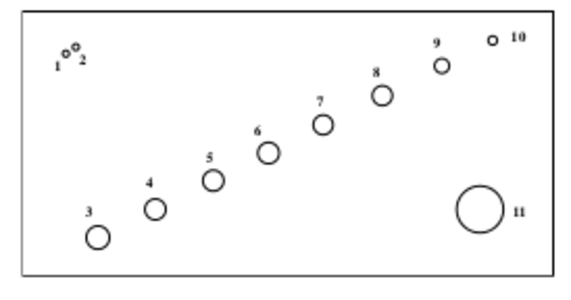
\includegraphics[width=0.7\textwidth]{Bilder/Block.pdf}
	\caption{Anordnung der Materialfehler im Acryl-Block.} %\cite{skript}} 
\label{fig:block}
\end{figure}
\begin{itemize}
\item{A-Scan}

Mit der $\SI{2}{\mega\hertz}$-Sonde wird die Laufzeit des Schalls mittels Echo-Impuls-Verfahren von beiden Seiten des Quaders gemessen. Dazu wird die Sonde über den Block geführt und $\Delta{t}$ jeweils für ein Loch notiert. Als Kontaktmittel dient Wasser.
\item{B-Scan}
Mit allen drei Sonden wird der B-Scan durchgeführt. Dazu werden die Sonden nacheinander langsam über den Quader geführt, sodass das Messprogramm ein 2-dimensionales Schnittbild entwirft.
\end{itemize}
\subsection{Augenmodell}
Ein Augenmodell wie in Abbildung \ref{fig:auge} wird mit dem A-Scan und der $\SI{2}{\mega\hertz}$-Sonde untersucht. Dazu wird das Kontaktgel auf die Oberfläche aufgetragen und unter leichtem Druck die Sondenposition so lange variiert, bis vier klar erkennbare Maxima auftreten. Diese entsprechen der Reflixion des Schalls an der Iris, den zwei Seiten der Linse und der Retina. Ein Bild des A-Scans wird aufgenommen und die Zeiten $\Delta{t}$ abgelesen.
\begin{figure}
	\centering
	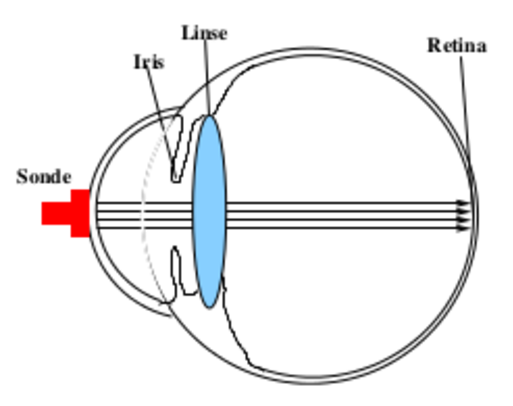
\includegraphics[width=0.5\textwidth]{Bilder/Auge.pdf}
	\caption{Augenmodell.}% \cite{skript}} 
\label{fig:auge}
\end{figure}

